\documentclass{article}
\usepackage{graphicx} % Required for inserting images
\usepackage{float}
\begin{document}
\boldmath
\section{me22b227}
\subsection{Details}
\begin{itemize}
    \item Mahendra Kurup
    \item ME22B227 (old: AE22B106)
    \item jellyfish2004
\end{itemize}
    
\subsection{Equation \cite{enwiki:1160233109}} 
\large
\[\frac{\partial^{2}{u}}{\partial{t}^2}=c^2(\frac{\partial^2 u}{\partial x_1 ^2}+\frac{\partial^2 u}{\partial x_2 ^2}+\ldots+\frac{\partial^2 u}{\partial x_n ^2}) \] 
\normalsize
\noindent The above equation is a second order differential equation which describes waves or standing wave fields.\footnote{URL : https://en.wikipedia.org/wiki/Wave\_equation}
Here,
\newline
\newline$u$ - is the function of the wave itself, i.e. the amplitude of the disturbance at any given point in space and time
\newline$t$ - represents time
\newline$x_1, x_2, \ldots, x_n$ - the coordinates in n-dimensions
\newline$c$ - A non-negative real constant, which represents the speed of the wave
\newline
\newline Using notations of Newtonian mechanics and vector calculus, it can be more compactly written as:
\[\ddot u = c^2 \nabla^2 u\]
For a normal sinusoidal wave, with speed $v$, wavelength $\lambda$, wave number $k$, angular frequency $\omega$, time period $T$, the plot looks like this:
\begin{figure}[H]
    \centering
    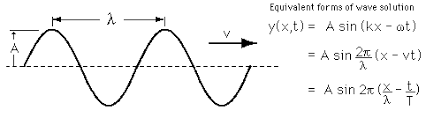
\includegraphics[width=10 cm]{wave.png}
    \caption{Sinusoidal wave}
    \label{fig:enter-label}
\end{figure}

\subsection{Derivation}
First, all waves can be written in the form of $u(x-ct)$ in one dimension, or more generally, $u(\vec{r}-\vec{c}t)$, where $\vec{r}= x_1 \hat{e_1} + x_2 \hat{e_2}+\ldots + x_n \hat{e_n}$ is the position in space, and $\vec{c}$ is the speed of the wave. I will derive the differential form for one dimension.
\newline This representation essentially means that if the amplitude of the wave is $u_0$ at $(r_0, t_0)$, then at a time $t+t_0$, it will have the value $u_0$ at $\vec{r}+\vec{c}t_0$. This shows the propagation of the wave in space. 
\newline Then, using the chain rule, the second derivative of the wave with respect to time can be written as:
\begin{equation}
    \frac{\partial ^2 u}{\partial t^2} = \frac{\partial ^2(u(x-ct))}{\partial (x-ct)^2}|c|^2
\end{equation}
\noindent And, after simplification, the second derivative with respect to $x$ is:
\begin{equation}
    \frac{\partial^2 u}{\partial x^2} = \frac{\partial ^2(u(x-ct))}{\partial (x-ct)^2}
\end{equation}
Using (1) and (2), we obtain:
\begin{equation}
    \frac{\partial^{2}{u}}{\partial{t}^2}=c^2\frac{\partial^2 u}{\partial x ^2}
\end{equation}
And for a wave in n-dimensions, we get:
\begin{equation}
    \frac{\partial^{2}{u}}{\partial{t}^2}=c^2(\frac{\partial^2 u}{\partial x_1 ^2}+\frac{\partial^2 u}{\partial x_2 ^2}+\ldots+\frac{\partial^2 u}{\partial x_n ^2})
\end{equation}
\subsection{Additional Info}
In the course PH1020, we have a chapter on electromagnetic waves, where we learnt about the second order partial differential equation described above. I found it interesting how there exists a general equation like this, because I was confused as to how we could express waves of any form, not just sinusoidal, with a general equation. That's why I picked this. I found more information on wikipedia, on how to obtain a general solution to the differential equation for any n number of dimensions, along with some more information, like dealing with problems at boundaries of two media. 

\bibliographystyle{plain}
\bibliography{refs.bib}

\end{document}
